%%
%% This is file `sample-acmtog.tex',
%% generated with the docstrip utility.
%%
%% The original source files were:
%%
%% samples.dtx  (with options: `acmtog')
%% 
%% IMPORTANT NOTICE:
%% 
%% For the copyright see the source file.
%% 
%% Any modified versions of this file must be renamed
%% with new filenames distinct from sample-acmtog.tex.
%% 
%% For distribution of the original source see the terms
%% for copying and modification in the file samples.dtx.
%% 
%% This generated file may be distributed as long as the
%% original source files, as listed above, are part of the
%% same distribution. (The sources need not necessarily be
%% in the same archive or directory.)
%%
%%
%% Commands for TeXCount
%TC:macro \cite [option:text,text]
%TC:macro \citep [option:text,text]
%TC:macro \citet [option:text,text]
%TC:envir table 0 1
%TC:envir table* 0 1
%TC:envir tabular [ignore] word
%TC:envir displaymath 0 word
%TC:envir math 0 word
%TC:envir comment 0 0
%%
%%
%% The first command in your LaTeX source must be the \documentclass command.
\documentclass[acmtog]{acmart}

%%
%% \BibTeX command to typeset BibTeX logo in the docs
\AtBeginDocument{%
  \providecommand\BibTeX{{%
    \normalfont B\kern-0.5em{\scshape i\kern-0.25em b}\kern-0.8em\TeX}}}

%% Rights management information.  This information is sent to you
%% when you complete the rights form.  These commands have SAMPLE
%% values in them; it is your responsibility as an author to replace
%% the commands and values with those provided to you when you
%% complete the rights form.
% \setcopyright{acmcopyright}
% \copyrightyear{2018}
% \acmYear{2018}
% \acmDOI{10.1145/1122445.1122456}


%%
%% These commands are for a JOURNAL article.
% \acmJournal{TOG}
% \acmVolume{37}
% \acmNumber{4}
% \acmArticle{111}
% \acmMonth{8}

%%
%% Submission ID.
%% Use this when submitting an article to a sponsored event. You'll
%% receive a unique submission ID from the organizers
%% of the event, and this ID should be used as the parameter to this command.
%%\acmSubmissionID{123-A56-BU3}

%%
%% The majority of ACM publications use numbered citations and
%% references.  The command \citestyle{authoryear} switches to the
%% "author year" style.
%%
%% If you are preparing content for an event
%% sponsored by ACM SIGGRAPH, you must use the "author year" style of
%% citations and references.
\citestyle{acmauthoryear}

%%
%% end of the preamble, start of the body of the document source.
\begin{document}

%%
%% The "title" command has an optional parameter,
%% allowing the author to define a "short title" to be used in page headers.
\title{A Tiny World: Atom}

%%
%% The "author" command and its associated commands are used to define
%% the authors and their affiliations.
%% Of note is the shared affiliation of the first two authors, and the
%% "authornote" and "authornotemark" commands
%% used to denote shared contribution to the research.
\author{Chung An, Chen}
\author{Yang, Liu}
\author{Linxi, Tao}

%%
%% By default, the full list of authors will be used in the page
%% headers. Often, this list is too long, and will overlap
%% other information printed in the page headers. This command allows
%% the author to define a more concise list
%% of authors' names for this purpose.

%%
%% The abstract is a short summary of the work to be presented in the
%% article.


%%
%% The code below is generated by the tool at http://dl.acm.org/ccs.cfm.
%% Please copy and paste the code instead of the example below.
%%

%%
%% This command processes the author and affiliation and title
%% information and builds the first part of the formatted document.
\keywords{Taichi, Atom, 3D, Rendering, Electron Cloud}
\maketitle

\section{Introduction}
Prior to the electron cloud model, there are a lot of attempts on building a theoretical model for an atom. Most of them, for example, the commonly known Rutherford-Bohr model, perceive the electrons as if they are planets orbiting the sun --- a non-changing centripetal movement. The electron cloud, however, models an atom consisting of a small, yet massive when put aside to its electrons, nucleus surrounded by a non-deterministic cloud of electrons.

In the electron cloud model, electrons can theoretically be found anywhere in the space. However, they are generally found more often in some regions, which we usually call them orbitals despite no orbital motions of electrons are being held, than others. A Carbon atom has two orbitals with the inner layer contains two electrons and the outer layer contains four. Electrons are less likely to be found in between layers.

This project aims to simulate and render a Carbon atom's presence in a three-dimensional space. The simulation will be grounded in the more accurate electron cloud model, shown in Figure 1 below. An electron cloud model depicts the occurence of an atom's electrons by a density map containing numerous sparse dots. In any region, the density of the dots draws a directly proportional relationship to the probability of an electron being present. To illustrate this model, We leverage a recently-built parallel programming language, namely \textbf{Taichi} \cite{hu2019taichi}, as our main development framework.

\begin{figure}[h]
  \centering
  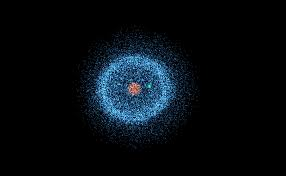
\includegraphics[width=\linewidth]{./concept_1.jpeg}
  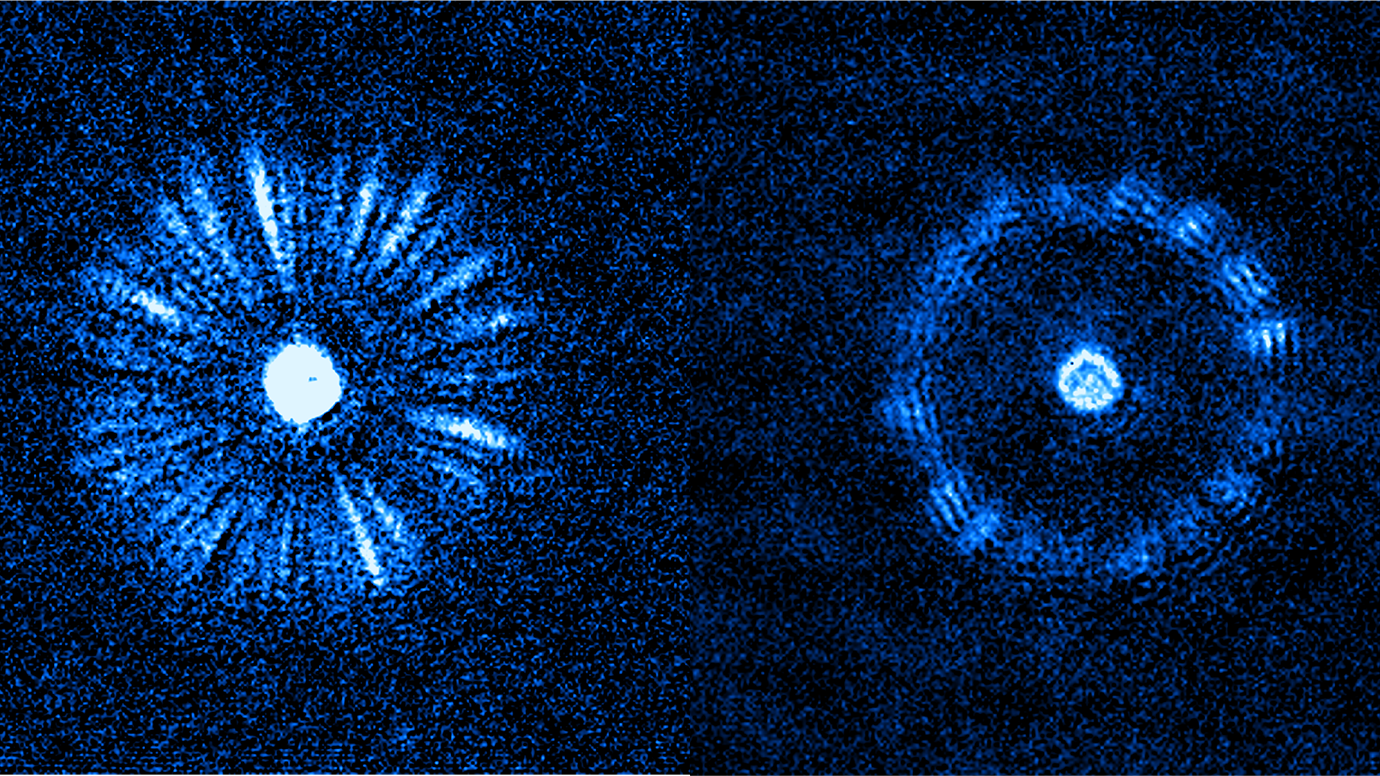
\includegraphics[width=\linewidth]{./concept_2.png}
  \caption{Atoms and Their Nucleus and Electron Cloud}
\end{figure}

\section{Software}
\textbf{Taichi} is a Python-based Domain-Specific Language designed for differentiable programming and speed up computer graphics development without compromising too much rendering performance. Despite inheriting most of its syntax from Python, \textbf{Taichi} relies on mostly parallel programming and does not carry over the downsides, for example, the slow computation speed, from Python.

\textbf{Taichi} is a higher level language such that it can be made to run on multiple mainstream rendering backends such as OpenGL, CUDA, and Metal. Using Pythonic decorators such as @ti.kernel and @ti.func brings the succeeding block of code into \textbf{Taichi}'s scope, where functions are naturally parallelized and differentiable on CPU or GPU devices. Two main data types in \textbf{Taichi} are Primitive Types and Compound Types. Primitive Types are numerical data types used by backends, while Compound Types are user-defined types composed of multiple members. To bridge across \textbf{Taichi}'s scope and Python's Scope, we use a global variable object called Field. They can correspond to OpenGL's vectors or matrices depending on how users define them.

\section{Code and Development}
We decided to proceed with render a Carbon atom to represent the main topic of our work. However, we can easily scale up or down by editting the code to render other atoms as they only differ by the number of protons, neutrons, electrons, and the layers of the electron cloud. 

For the prototype shown in Figure 2, we started off by using a simple ray-marching model and shattered beams of light of extremely small radius towards the protons and neutrons. Instead of directly specifying the layers of electron cloud, we manipulate shadow of the protons and neutrons and use them to form a relatively hollow region to represent the sparseness of the electrons. In the outer region, the light beams are able to fully hit the back of the wall and thus generating a denser cloud of electrons.

\begin{figure}[h]
  \centering
  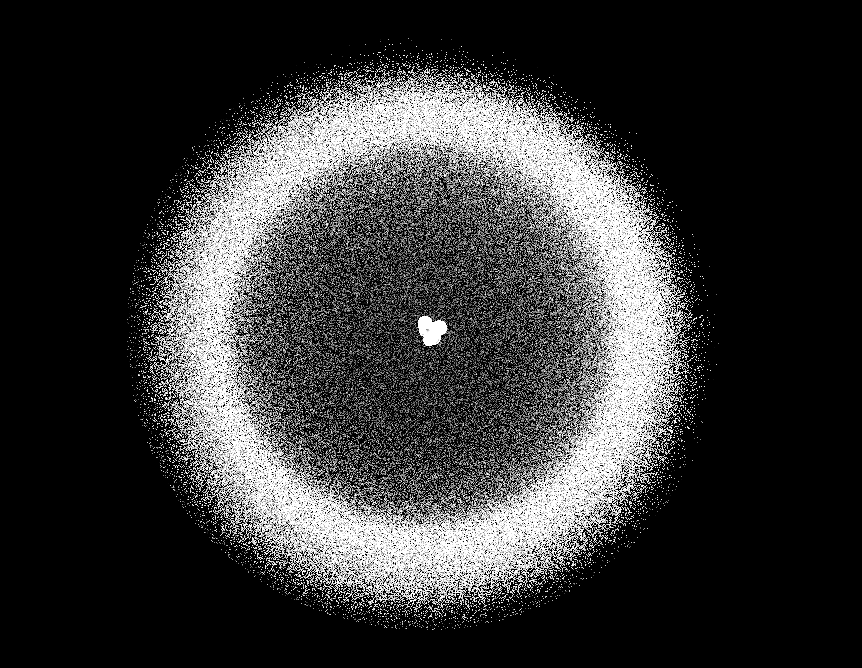
\includegraphics[width=\linewidth]{./prototype.png}
  \caption{Ray-marching Prototype}
\end{figure}

However, we did not proceed with the prototype as the layers of electrons cloud are not scalable.

For the next step, we decided to proceed with rendering protons, neutrons, and electron clouds using tiny particles. We abide the physics observations and define protons and neutrons to be roughly equal size of round particles, with neutrons being slightly larger, of size around 0.05. We do not render the electrons since they only possess mass and charge. We use particles that are ten times smaller just to depict the electron cloud.

\begin{figure}[h]
  \centering
  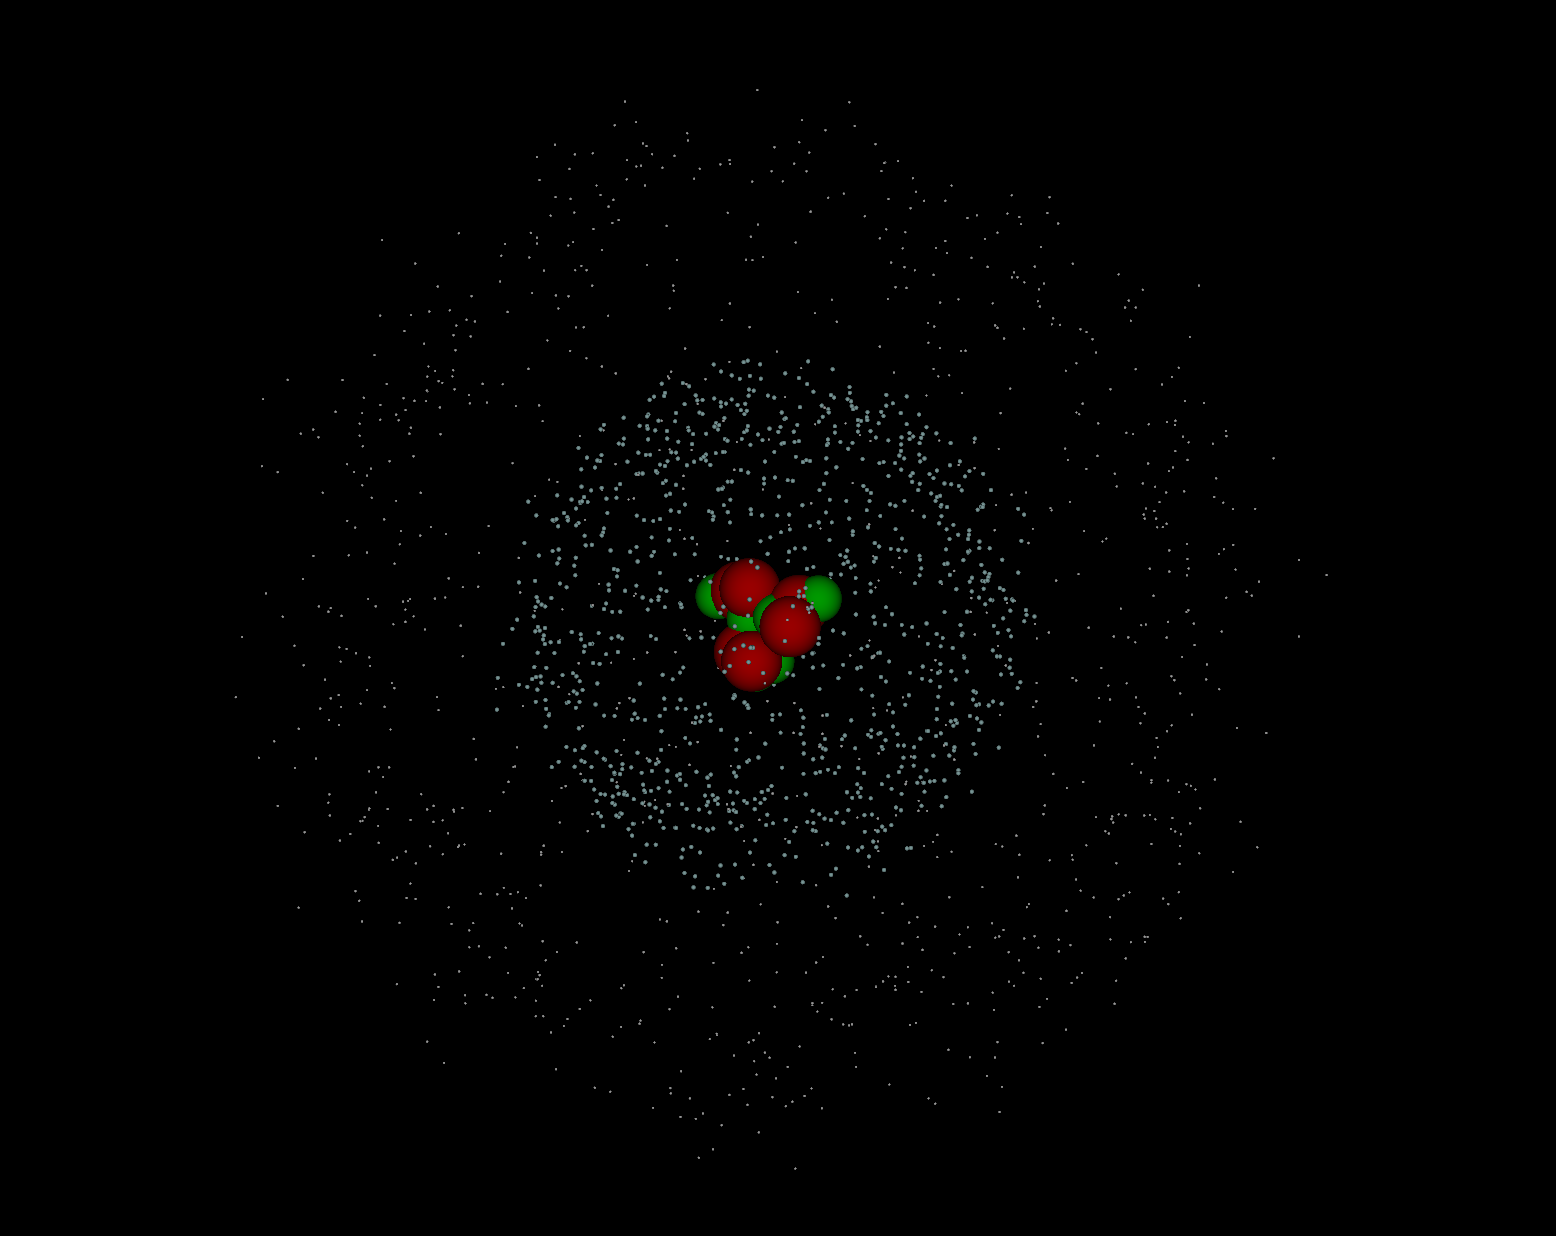
\includegraphics[width=\linewidth]{./carbon.png}
  \caption{A (Rotating) Carbon Atom}
\end{figure}

We set the electron clouds to two different colors just to make the image more friendly to human eyes. In the center we have six protons and six neutrons rendered green and red respectively. There are two hollow spaces in the image with one located in between the inner electron cloud layer and the neucleus and the other located between the two layers of electron cloud. This is because the energy that an electron can emit or absorbed is quantized, and thus electrons can only appear in specific levels of orbit. 

\begin{figure}[h]
  \centering
  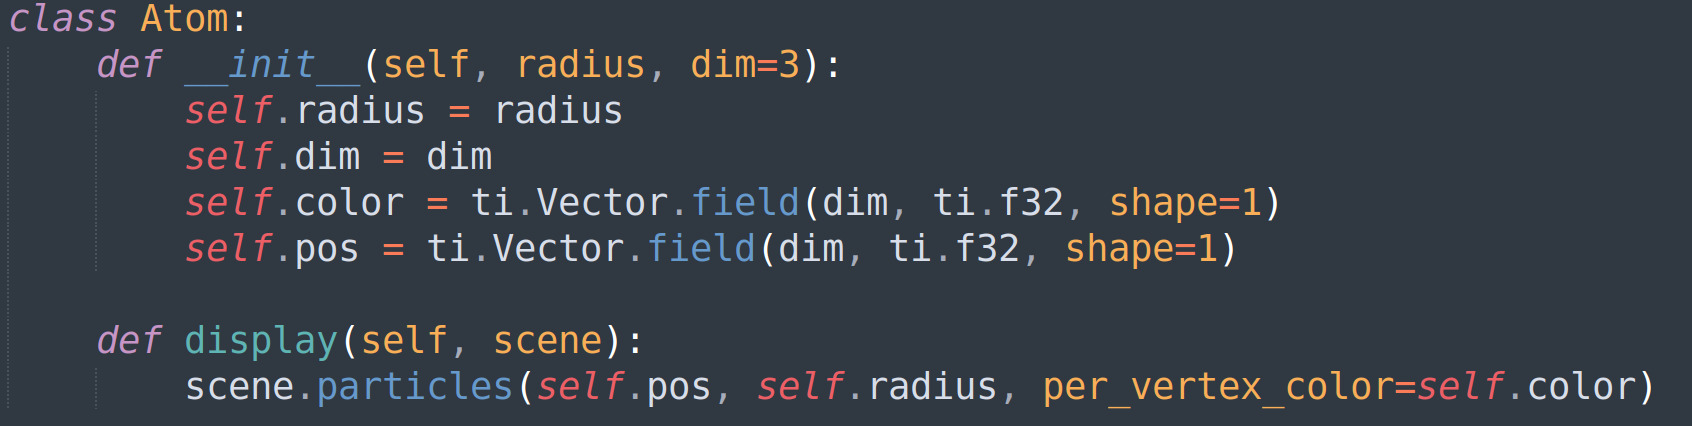
\includegraphics[width=\linewidth]{./atom.png}
  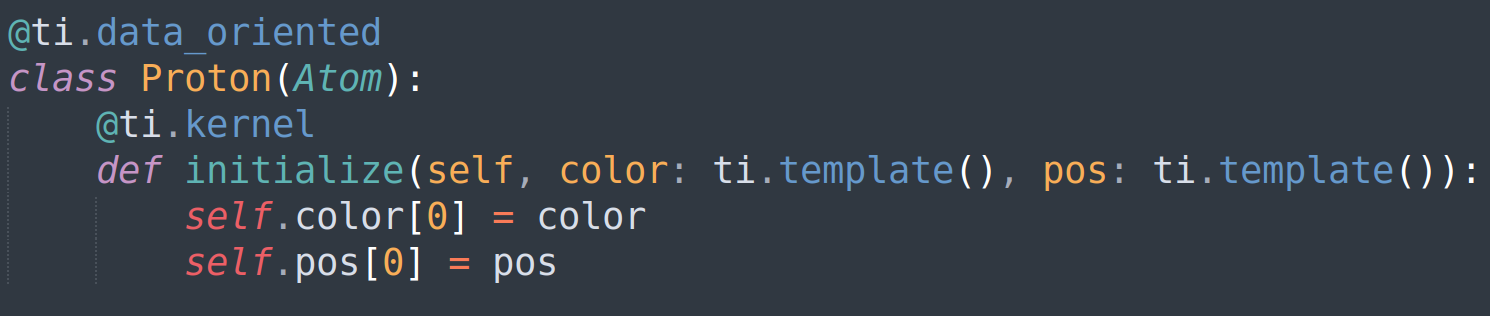
\includegraphics[width=\linewidth]{./proton.png}
  \caption{Particle Implementation}
\end{figure}

Figure 4 shows the general implementation of a single proton, neutron, and electron particle. We simply render them as spherical objects with different sizes and colors. In reality, protons tend to repel each other and attract neutrons. Therefore, in our implementation, we try to pair protons to neutrons so that protons are not clustered and are some what distant apart.

\begin{figure}[h]
  \centering
  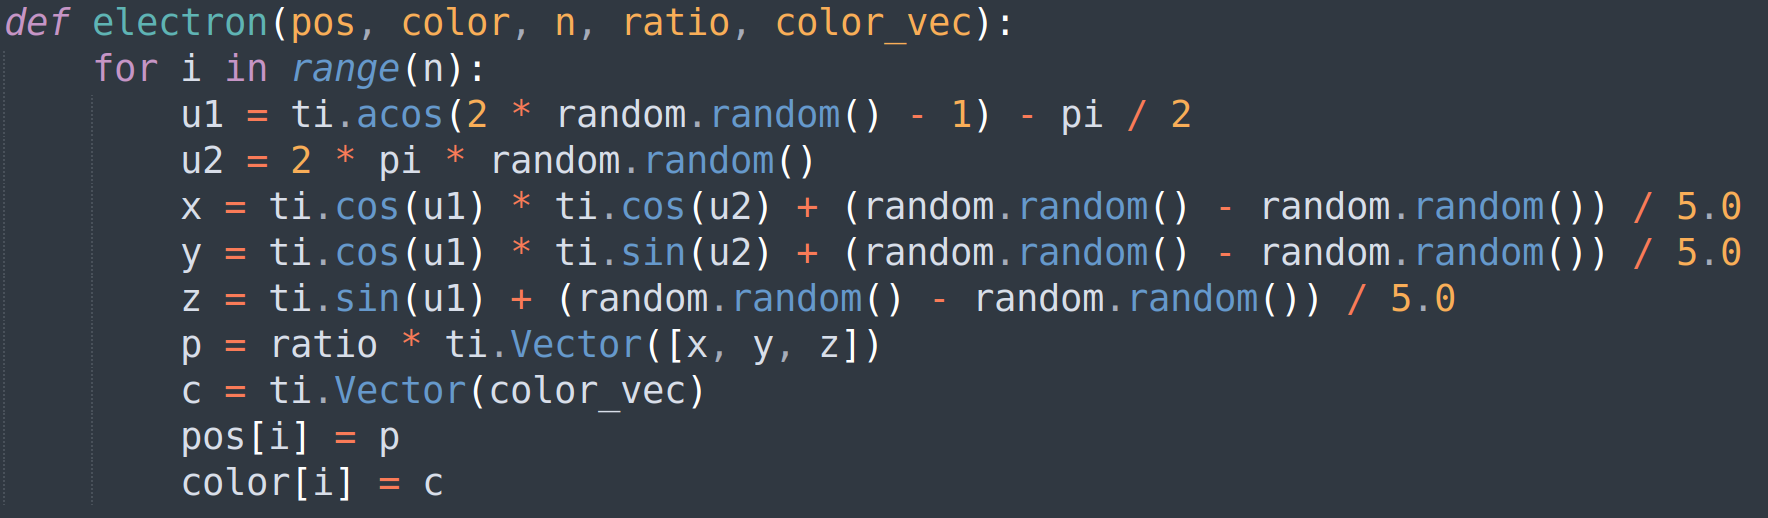
\includegraphics[width=\linewidth]{./electron_cloud.png}
  \caption{Electron Cloud}
\end{figure}

Figure 5 shows the formation of shells of electron clouds. Randomness is added to not only distribute them across the shell but also to level electrons on the same shell unevenly.

\begin{figure}[h]
  \centering
  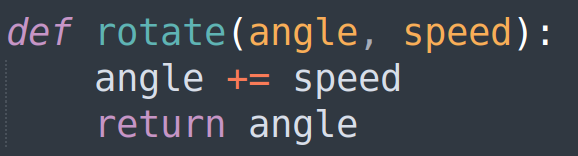
\includegraphics[width=\linewidth]{./rotate.png}
  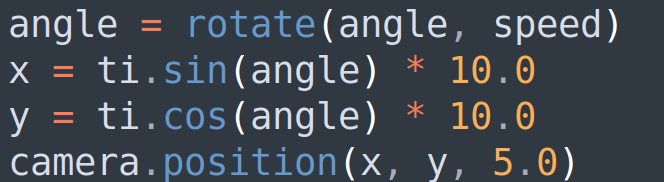
\includegraphics[width=\linewidth]{./camera.png}
  \caption{Rotation Implementation}
\end{figure}

Figure 6 shows how we rotate the camera to mimic the rotation of the atom instead of giving each partical a velocity and acceleration, which is extremely computationally expensive.

\begin{figure}[h]
  \centering
  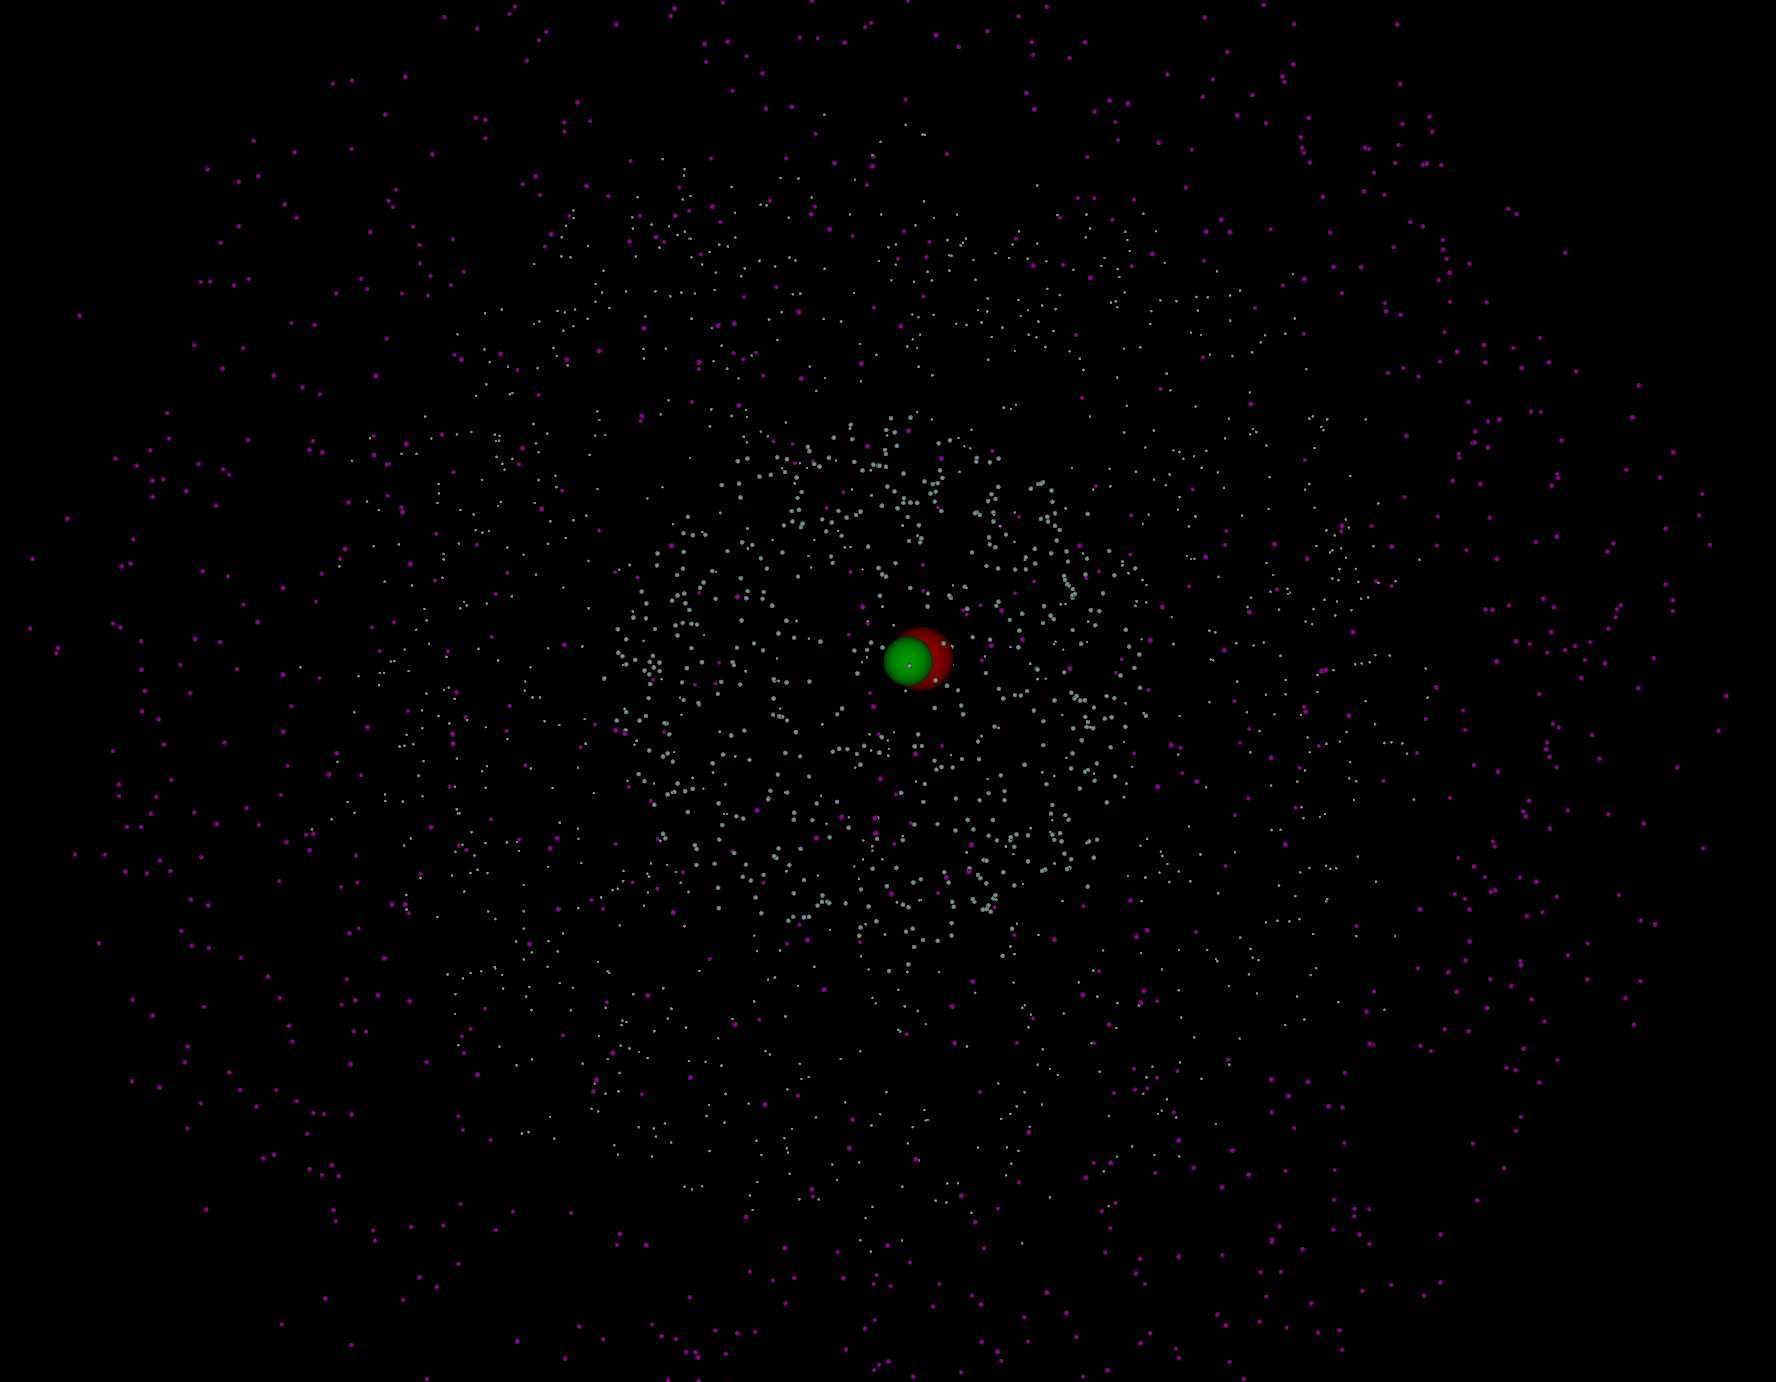
\includegraphics[width=\linewidth]{./example.png}
  \caption{A Different Example}
\end{figure}


Figure 7 is an example another implementation with differnt hyperparamters, namely an imaginary atom containing a neucleus of one proton and one neutron with three layers of electron clouds.

\section{Source}
All of our work can be found here \href{https://github.com/andy971022/acg-project}{https://github.com/andy971022/acg-project}.



\bibliographystyle{ACM-Reference-Format}
\bibliography{acmart}

\end{document}



\endinput
%%
%% End of file `sample-acmtog.tex'.
